\section{本次里程碑任务}
\begin{frame}
    \frametitle{本次里程碑任务}
    \begin{itemize}
        \item 确定项目开发技术栈,搭建项目开发环境,使得相关框架能够正确集成并且运行。
        \item 根据甲方项目需求SRS文档,完成项目的需求分析,确定项目的主要功能,完成项目的功能设计与主要功能模块划分。
        \item 完成项目软件架构的逻辑设计和物理设计,主要包括数据库schema设计、索引设计、存储过程设计和视图设计,基于Restful API接口规范进行后端接口路由和功能设计等。
        \item 基于上述设计内容,使用华为云平台进行版本管理,将大功能模块设置为EPIC工作项,并且在Epic下抽取Feature,对于每个Feature进一步划分User Story,并且确定第一次迭代中需要实现的用户故事,最后分配工作到每位组员进行代码开发。
    \end{itemize}
\end{frame}

\begin{frame}
    \frametitle{工作项总览}
    我们小组在项目启动会中根据上述里程碑任务计划,详细讨论了项目的需求分析、软件架构设计、项目管理等内容,将设计细节落实到华为云工作项和开发文档,最终确定了本次里程碑任务的工作项,如下图所示:
        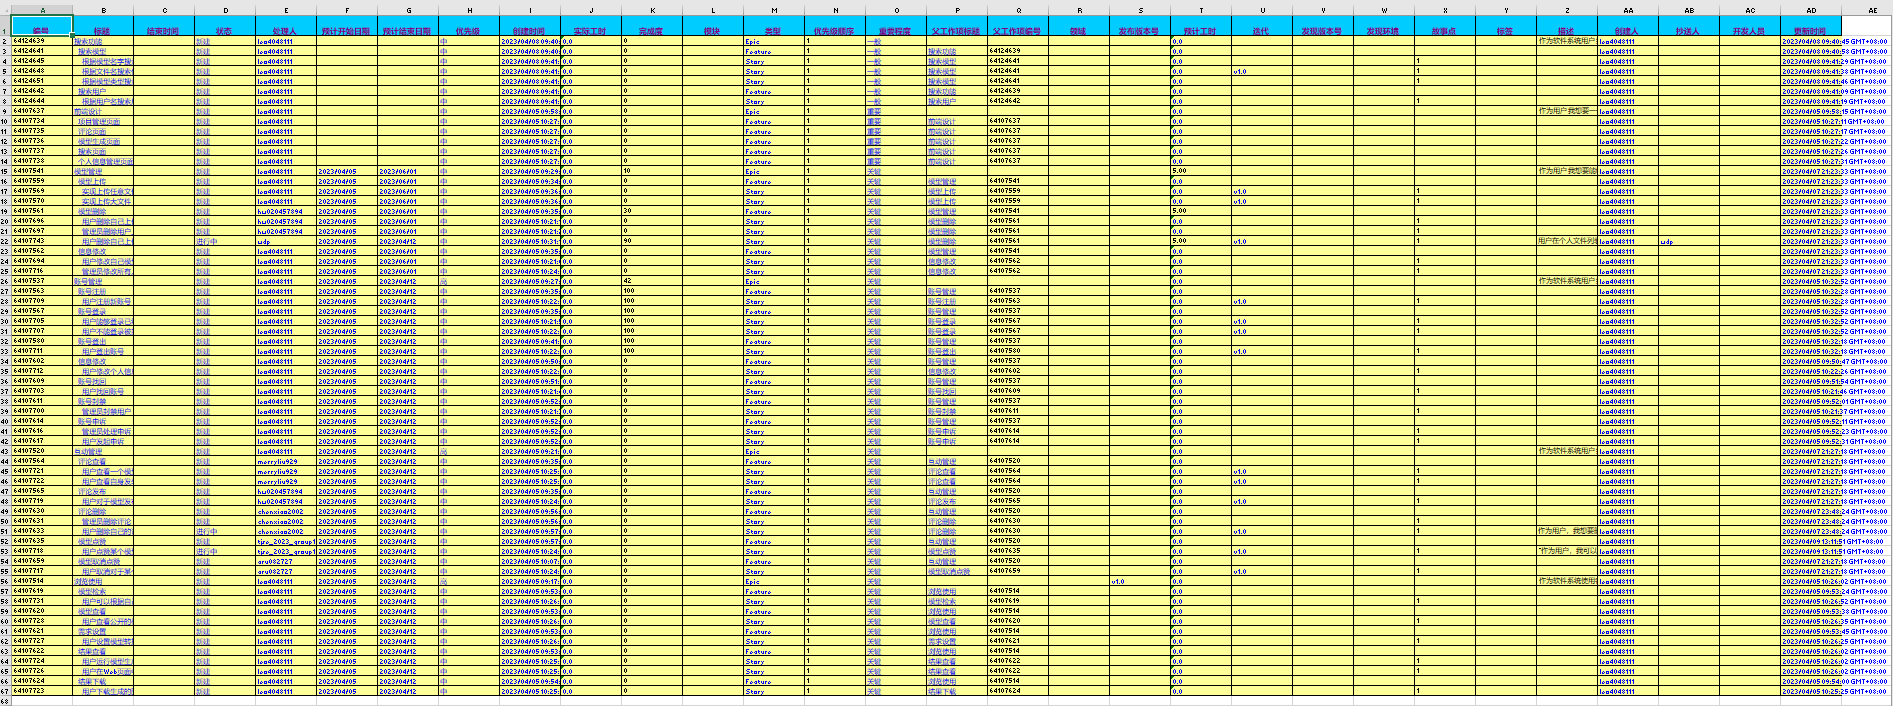
\includegraphics[width=2\textwidth]{contents/figure/work_items_overall.png}
\end{frame}


\begin{frame}
    \frametitle{项目技术栈}
    \begin{itemize}
        \item 主要开发语言:Python + HTML + CSS(SCSS) + JavaScript(Vue.js)
        \item HTTP服务器:Tornado
        \item 持久层框架:SQLAlchemy
        \item 数据库服务:MySQL + Redis
        \item 版本管理工具:Git
        \item 远程代码托管平台:华为云
        \item 接口管理与自动化测试工具:Apifox + Mock.js
    \end{itemize}
\end{frame}